\documentclass{beamer}
\usepackage{beamerthemesplit}
\usepackage{wrapfig}
\usetheme{SPbGU}
\usepackage{pdfpages}
\usepackage{amsmath}
\usepackage{cmap} 
\usepackage[T2A]{fontenc} 
\usepackage[utf8]{inputenc}
\usepackage[english,russian]{babel}
\usepackage{indentfirst}
\usepackage{amsmath}
\usepackage{tikz}
\usepackage{multirow}
\usepackage[noend]{algpseudocode}
\usepackage{algorithm}
\usepackage{algorithmicx}
\usetikzlibrary{shapes,arrows}
\usepackage{fancyvrb}
\usepackage{appendixnumberbeamer}
\usepackage{xcolor,colortbl}
\usepackage{listings}
\usepackage{multicol}
\usepackage{tabularx}

\newtheorem{rutheorem}{Теорема}
\newtheorem{ruproof}{Доказательство}
\newtheorem{rudefinition}{Определение}
\newtheorem{rulemma}{Лемма}

\definecolor{mygreen}{rgb}{0,0.6,0}
\definecolor{mygray}{rgb}{0.5,0.5,0.5}
\definecolor{mymauve}{rgb}{0.58,0,0.82}

\lstset{ %
  backgroundcolor=\color{white},   % choose the background color
  basicstyle=\footnotesize,        % size of fonts used for the code
  breaklines=true,                 % automatic line breaking only at whitespace
  captionpos=b,                    % sets the caption-position to bottom
  commentstyle=\color{mygreen},    % comment style
  escapeinside={\%*}{*)},          % if you want to add LaTeX within your code
  keywordstyle=\color{blue},       % keyword style
  stringstyle=\color{mymauve},     % string literal style
  captionpos=b,
  frame=single
}

\beamertemplatenavigationsymbolsempty

\title[GraphBLAS F\#]{Высокоуровневая реализация спецификации GraphBLAS с поддержкой исполнения на GPU}
\institute[СПбГУ]{}
\author[Панфилёнок Дмитрий]{Панфилёнок Дмитрий Викторович,  18.Б10-мм группа}
 
\begin{document}
{
\setbeamertemplate{footline}{}
\begin{frame}
  
\includegraphics[width=1.4cm]{pictures/SPbGU_Logo.png}
\vspace{-35pt}
\hspace{-10pt}
\begin{center}
  \begin{tabular}{c}
    \scriptsize{Санкт-Петербургский государственный университет} \\
    \scriptsize{Кафедра системного программирования}
    \end{tabular}
\titlepage
\end{center}

\btVFill

{\scriptsize{\bfseries Научный руководитель:} к.ф.-м.н., доцент кафедры информатики С.В. Григорьев \\ }

\begin{center}
  \vspace{5pt}
  \scriptsize{Санкт-Петербург\\
                 2021}
  \end{center}
\end{frame}
}

\begin{frame}[fragile]  
  \frametitle{Введение}
  \begin{itemize}
  	\item Графы могут быть представлены разреженными матрицами
  	\item Алгоритмы на графах можно выразить в терминах линейной алгебры над различными полукольцами
    \item Спецификация GraphBLAS описывает структуру объектов и методов для реализации таких алгоритмов в терминах линейной алгебры
  \end{itemize}
  \begin{figure}
    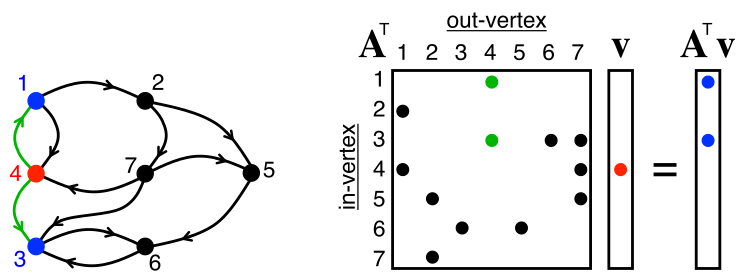
\includegraphics[scale=0.35]{pictures/MatrixBFS.png}
    \caption{Вычисление одного шага в алгоритме поиска в ширину\footnotemark}
  \end{figure}
  \footnotetext{GraphBLAS [Электронный ресурс] // Википедия. Свободная энциклопедия. – URL: \url{https://en.wikipedia.org/wiki/GraphBLAS} (дата обращения: 13.12.2020).}
\end{frame}
     
\begin{frame}  
  \frametitle{Существующие решения}
  \begin{table}[htbp]
    \begin{tabularx}{\textwidth}{X|X|l}
      Реализация & Язык & Поддержка GPU \\
      \hline
      SuiteSparse & C & Нет \\
      GBTL & C++ & Нет (версия с CUDA устарела) \\
      GraphBLAST & C++ & CUDA \\
      CombBLAS & C++ & Частичная, CUDA \\
      Graphulo & Java & Нет \\ 
      \hline
    \end{tabularx}
  \end{table}
  
  \bigskip
  \textbf{Недостатки существующих решений:}
  \begin{itemize}
    \item GraphBLAS на GPU --- открытая проблема
  	\item Низкая переносимость решений, основанных на CUDA
    \item Нет самостоятельных библиотек для высокоуровневых языков
  \end{itemize}
\end{frame}

\begin{frame}
  \frametitle{Постановка задачи}
  \textbf{Целью} данной работы является реализация высокоуровневой, производительной и переносимой библиотеки на основе стандарта GraphBLAS.
  
  ~\\
  \textbf{Задачи:}
  \begin{itemize}
    \item Реализовать структуру объектов и методов, соответствующих спецификации GraphBLAS
    \item Реализовать базовые примитивы линейной алгебры для выполнения на устройствах с поддержкой GPGPU
    \item Провести экспериментальное исследование предложенной реализации и сравнить её с аналогичными решениями в предметной области
  \end{itemize}
\end{frame}

\begin{frame}  
  \frametitle{Обзор инструментов}
%   что то из этого можно убрать со слайда и просто проговорить
  \textbf{Программные интерфейсы для GPGPU:}
  \begin{itemize}
    \item CUDA
  	\item OpenCL
    \item Metal
  \end{itemize}
  \bigskip
  \textbf{Поддержка OpenCL в .NET и Java:}
  \begin{table}[htbp]
  \begin{tabularx}{\textwidth}{X|X}
    .NET & Java \\
    \hline
    OpenCL.NET & JavaCL \\
    Cloo & JOCL \\
    FSCL & Aparapi \\
    Brahma.FSharp & ScalaCL \\
    \hline
  \end{tabularx}
  \end{table}
\end{frame}

\begin{frame}  
  \frametitle{Предлагаемое решение}
  \begin{figure}
    
\includegraphics[scale=0.2]{pictures/impl1.png}
  \end{figure}
\end{frame}
       
\begin{frame}[fragile]
  \frametitle{Стандарт GraphBLAS}
    \begin{itemize}
      \item Mатрицы, векторы
      \item Mоноиды, полукольца, бинарные и унарные операторы
      \item Mxm, vxm, mxv, eWiseAdd eWiseMult, reduce и другие
      \item Mаски, дескрипторы
    \end{itemize}
\end{frame}

\begin{frame}  
  \frametitle{Архитектура решения}
  \begin{figure}
    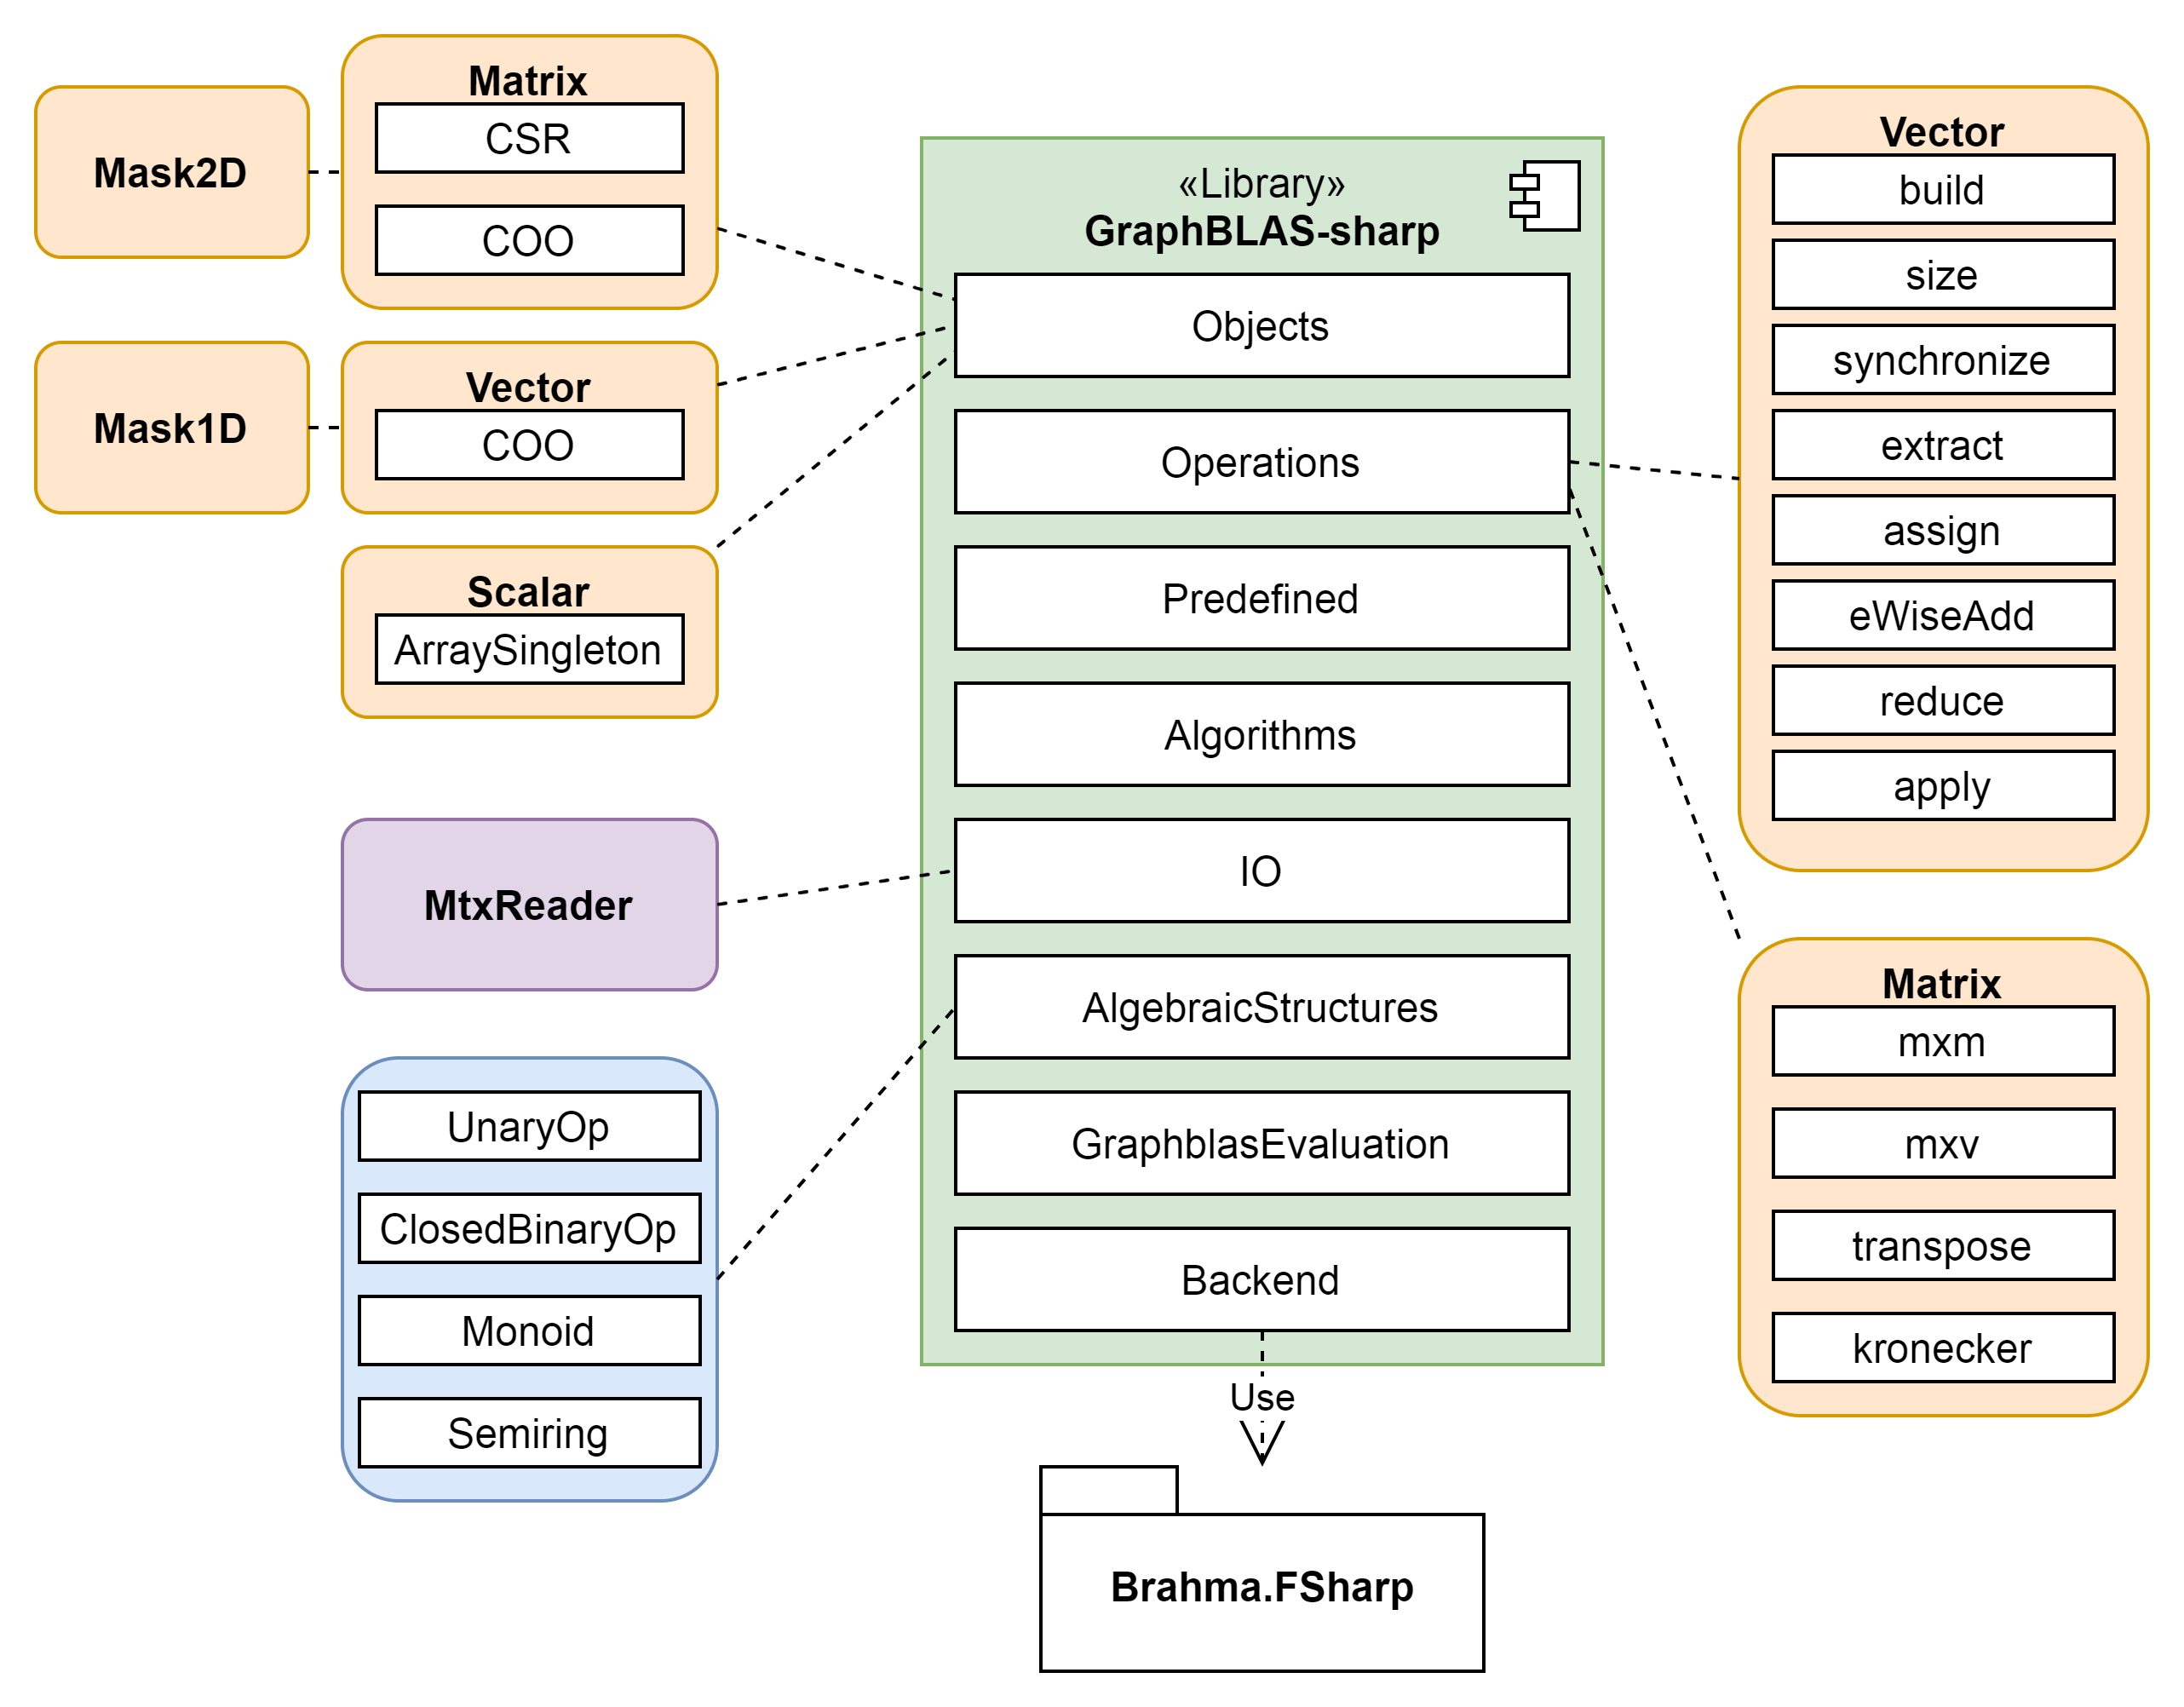
\includegraphics[scale=0.4]{pictures/dia3.png}
    \caption{Библиотека GraphBLAS-sharp}
  \end{figure}
\end{frame} 

\begin{frame}  
  \frametitle{Выбор алгоритмов для реализации операций}
  \begin{itemize}
    \item W. Liu and B. Vinter, "An Efficient GPU General Sparse Matrix-Matrix Multiplication for Irregular Data"\,, 2014\footnote{\url{https://ieeexplore.ieee.org/document/6877271}}
    \item Y. Nagasaka, A. Nukada and S. Matsuoka, "High-Performance and Memory-Saving Sparse General Matrix-Matrix Multiplication for NVIDIA Pascal GPU"\,, 2017\footnote{\url{https://ieeexplore.ieee.org/document/8025284}}
    \item Y. Tao et al., "Atomic reduction based sparse matrix-transpose vector multiplication on GPUs"\,, 2014\footnote{https://ieeexplore.ieee.org/document/7097920}
    \item Yang, Carl, Yangzihao Wang, and John D. Owens. "Fast sparse matrix and sparse vector multiplication algorithm on the gpu"\,, 2015\footnote{\url{https://escholarship.org/content/qt1rq9t3j3/qt1rq9t3j3.pdf}}
  \end{itemize}
\end{frame} 

\begin{frame} 
  \frametitle{Реализованные операции}
  \begin{itemize}
      \item Умножение матрицы в CSR формате на разреженный вектор 
      \begin{enumerate}
        \item Каждая строка матрицы умножается на разреженный вектор
        \item Получаем массив значений и массив, в котором для каждой строчки хранится количество произведений 
        \item Из полученного плотного вектора удаляются элементы, для которых число произведений в соответствующем массиве нулевое
      \end{enumerate}
      \item Транспонирование матрицы в CSR формате
      \begin{enumerate}
        \item Матрица в CSR формате конвертируется в формат COO
        \item Сортируются соответствующие массивы
        \item Матрица в COO формате конвертируется в формат CSR
      \end{enumerate}
  \end{itemize}
\end{frame} 
  
\begin{frame}  
  \frametitle{Эксперименты}
  \begin{table}[htbp]
    \begin{tabularx}{\textwidth}{X|l|l|X|X}
      Название & |V| & |E| & GraphBLAS-sharp, мс & QuickGraph, мс \\
      \hline
      arc130 & 130 & 1282 & 347.9 & 0.063 \\
      linux-call-graph & 324085 & 1208908 & 8765.3 & 9.6 \\
      webbase-1M & 1000005 & 3105536 & 9867.5 & 18.7 \\
      cit-Patents & 3774768 & 16518948 & 2888.4 & 136.6 \\ 
      \hline
    \end{tabularx}
  \caption{Медиана времени работы алгоритма поиска в ширину}
  \end{table}
  \begin{itemize}
    \item Windows 10, Intel Core i5-4690K CPU 3.50GHz, DDR3 8GB RAM, GeForce GTX 970, 4GB VRAM
  \end{itemize}
\end{frame} 
      
\begin{frame}  
  \frametitle{Выводы и ограничения подхода}
  \begin{itemize}
    \item Managed $\longrightarrow$ Native $\longrightarrow$ GPU 
    \item Компиляция во время исполнения может занимать много времени
    \item Нет атомарных операций
    \item Сложно профилировать
  \end{itemize}
\end{frame}
             
\begin{frame}  
  \frametitle{Результаты}
  \begin{itemize}
    \item Реализована\footnote{Репозиторий решения: \url{https://github.com/YaccConstructor/GraphBLAS-sharp}} структура объектов и методов GraphBLAS на языке F\#
    \item Реализовано подмножество операций линейной алгебры для выполнения на устройствах с поддержкой OpenCL
    \begin{itemize}
      \item Умножение матрицы в CSR формате на разреженный вектор
      \item Транспонирование матрицы в CSR формате
    \end{itemize}
    \item Поставлены эксперименты и проведено сравнение предложенной реализации с аналогами
  \end{itemize}
\end{frame}         

\appendix

\begin{frame}[fragile]
  \frametitle{Приложение 1}
  \begin{lstlisting}[language=ml, caption=Реализация поиска в ширину в GraphBLAS-sharp, basicstyle=\tiny, numbers=left, numberstyle={\tiny \color{black}}, xleftmargin=5.0ex]
let levelSingleSource (matrix: Matrix<int>) (source: int) = graphblas {
    let vertexCount = Matrix.rowCount matrix
    let! levels = Vector.zeroCreate vertexCount
    let! frontier = Vector.ofList vertexCount [source, 1]
    let mutable currentLevel = 0
    let mutable break' = false
    while not break' do
        currentLevel <- currentLevel + 1
        let! currentLevelScalar = Scalar.create currentLevel
        let! frontierMask = Vector.mask frontier
        do! Vector.fillSubVector levels frontierMask currentLevelScalar
        let! levelsComplemented = Vector.complemented levels
        do! Matrix.mxvWithMask AddMult.int levelsComplemented transposed frontier
        >>= Vector.assignVector frontier
        let! succ =
            Vector.reduce AddMult.int frontier
            >>= Scalar.exportValue
        break' <- succ = 0
    return levels
}
  \end{lstlisting}
\end{frame}

\begin{frame}[fragile]
  \frametitle{Приложение 2}
  \begin{lstlisting}[language=c++, caption=Реализация поиска в ширину в GraphBLAST, basicstyle=\tiny, numbers=left, numberstyle={\tiny \color{black}}, xleftmargin=5.0ex]
void bfs(Vector<float> *v, const Matrix<float> *A, Index s, Descriptor *desc){
    Index A_nrows;
    CHECK(A->nrows(&A_nrows));
    CHECK(v->fill(0.f));
    Vector<float> q1(A_nrows);
    Vector<float> q2(A_nrows);
    std::vector<Index> indices(1, s);
    std::vector<float> values(1, 1.f);
    CHECK(q1.build(&indices, &values, 1, GrB_NULL));
    float iter = 1;
    float succ = 0.f;
    do {
        assign<float, float>(v, &q1, GrB_NULL, iter, GrB_ALL, A_nrows, desc);
        CHECK(desc->toggle(GrB_MASK));
        vxm<float, float, float, float>(
            &q2, v, GrB_NULL, LogicalOrAndSemiring<float>(), &q1, A, desc);
        CHECK(desc->toggle(GrB_MASK));
        CHECK(q2.swap(&q1));
        reduce<float, float>(&succ, GrB_NULL, PlusMonoid<float>(), &q1, desc);
        iter++;
    } while (succ > 0);
}
  \end{lstlisting}
\end{frame}

\begin{frame}[fragile]
  \frametitle{Приложение 3}
  \begin{lstlisting}[language=Python, caption=Реализация поиска в ширину в pygraphblas, basicstyle=\tiny, numbers=left, numberstyle={\tiny \color{black}}, xleftmargin=5.0ex]
def bfs(matrix, start):
    v = Vector.sparse(UINT8, matrix.nrows)  
    q = Vector.sparse(BOOL, matrix.nrows)    
    q[start] = True
    not_done = True
    level = 1
    while not_done and level <= matrix.nrows:
        v.assign_scalar(level, mask=q)          
        q = v.vxm(matrix, mask=v, 
                  desc=descriptor.ooco)         
        not_done = q.reduce_bool()              
        level += 1                              
    return v
  \end{lstlisting}
\end{frame}

\begin{frame}[fragile]
  \frametitle{Приложение 4}
  \begin{lstlisting}[language=ml, caption=GraphBLAS-sharp, basicstyle=\tiny]
// t4 <- sigma.[i - 1, *] * t3
do! Matrix.extractRow sigma (i - 1)
>>= Vector.apply (UnaryOp <@ float32 @>)
>>= fun x -> Vector.eWiseMult AddMult.float32 x t3
>>= Vector.assignVector t4
  \end{lstlisting}
  
  \begin{lstlisting}[language=c, caption=SuiteSparse GraphBLAS, basicstyle=\tiny]
// t4 = sigma[i - 1, :]
GrB_extract(t4, GrB_NULL, GrB_NULL, sigma, GrB_ALL, n, i - 1, GrB_DESC_T0);
// t4 = t4 * t3
GrB_eWiseAdd(*delta, GrB_NULL, GrB_NULL, GrB_PLUS_FP32, *delta, t4, GrB_NULL);
  \end{lstlisting}
\end{frame}

\begin{frame}  
  \frametitle{Приложение 5}
  \begin{table}[htbp]
    \begin{tabularx}{\textwidth}{X|l|l|X}
      Название & |V| & |E| & GraphBLAS-sharp, мс \\
      \hline
      arc130 & 130 & 1282 & 129.1 \\
      linux-call-graph & 324085 & 1208908 & 732.9 \\
      webbase-1M & 1000005 & 3105536 & 929.9 \\
      cit-Patents & 3774768 & 16518948 & 2091.9 \\ 
      \hline
    \end{tabularx}
  \caption{Среднее время работы алгоритма транспонирования}
  \end{table}
  \begin{itemize}
    \item Windows 10, Intel Core i5-4690K CPU 3.50GHz, DDR3 8GB RAM, GeForce GTX 970, 4GB VRAM
  \end{itemize}
\end{frame} 

\end{document}